\documentclass[journal,onecolumn]{IEEEtran}
\usepackage[utf8]{inputenc}
%\usepackage{hyperref}
\usepackage[sort,compress]{cite}
\usepackage{algorithmic}
\usepackage[ruled,linesnumbered,lined]{algorithm2e}
\usepackage{booktabs}

\usepackage{amsfonts}%Usando fontes para conjuntos numéricos

%\usepackage{titlesec}
\usepackage{color,colortbl,multirow}
\usepackage{xy}
\usepackage{graphicx,url, amsmath, color}
\usepackage{graphicx}
\usepackage{titling}

\newcommand{\subtitle}[1]{%
  \posttitle{%
    \par\end{center}
    \begin{center}\large#1\end{center}
    \vskip0.5em}%
}
\title{Relatorio de projeto de segunda VA}
\subtitle{Réplica do trabalho:Simple face-detection algorithm based on minimum facial features}
\author{		Ismael Cesar da Silva Araujo
  				Departamento de computação \\
				  Ciência da computação\\
		Universidade Federal Rural de Pernambuco (UFRPE)\\
			ismael.cesar@ufrpe.br}
\date{}
\begin{document}
\maketitle

\section{Introdução}

\section{Conceitos Básicos}
	\subsection{Detecção de pele}
	O modelo de cor normalizado, trata-se de um tipo de normalização feita por pixel. 
	Considerando uma com canais RGB (Sigla em inglês para Vermelho Verde e Azul), 
	A normalização da imagem segundo o modelo de cor normalizada calcularia pra cada pixel o valor contido no canal dividido pela soma de todos os valores dos canais no pixel avaliado~\cite{chen2007simple,loesdau2017chromatic}. 
	Seja $\varepsilon$ um valor da ordem de $10^{-8}$, somado a o denominador para se evitar divisão por zero\eqref{eq:nomalizedColorModel}.	
	\begin{equation}
		\begin{split}
			r  = \frac{R}{R+G+B+\varepsilon} \\\\
			g  = \frac{G}{R+G+B+\varepsilon} \\\\
			b  = \frac{B}{R+G+B+\varepsilon}
			\label{eq:nomalizedColorModel}
		\end{split}
	\end{equation}		
	A normalização das cores da imagem possibilitam a diminuição da sensibilidade do algorítmo de detecção em relação as variações de cores e illuminação.
	Normalizados os intervalos de valores do pixel, é necessário definir funções que avaliam os tons de vermelho  que foram normalizados.
	Tais funções são utilizadas para a definição dos limites superiores e inferiores do intervalo de tons de pele em relação ao canal $r$~\cite{soriano2000using,chen2007simple}.
	\begin{equation}
		\begin{split}
			F_1(r)  = -1.367r^2 + 1.0743r + 0.2 \\
			F_2(r)  = -0.776r^2 + 0.5601r + 0.18
		\end{split}
	\end{equation}
	
	Para o aprimoramento da detecção de pele necessário definir funções para avaliação de tons e branco, em conjunto com valores de matiz ou \textit{Hue} do píxel.
	A avaliação dos tons de branco é feita segundo os valores dos canais $r$ e $g$ do píxel. 
	De modo que o píxel é considerado com algum tom de branco quando $r=0.33$ e $g=0.33$~\cite{chen2007simple}.
	Onde a diferença dos valores dos canais $r$,$g$ e $0.33$ é elevada ao quadrado para para que a mesma só retorne o valor absoluto caso $r$ e $g$ possuam valores menores que $0.33$.
	
	\begin{equation}
		White(r,g) = (r - 0.33)^2 + (g - 0.33)^2 
		\label{eq:whiteValue}
	\end{equation}
	
	Para se constar se o píxel em questão tem algum tom de branco, verifica-se o resultado da comparação entre $White(r,g) > 0.001$.
	Para melhorar o desempenho da detecção de pele é necessário computar a relação entre o modelo de cor HSI (Hue Saturation and Itensity) com o modelo RGB.
	Onde \textit{Hue} descreve a cor que está sendo utilizada, o valor está no intervalo em $[0,360]$ o qual representa o ângulo no circulo unitário.
	\textit{Saturation} representa o nível de puresa da cor, e \textit{Intensity} trata-se de um valor acromático , que representa a itesidade da cor.
	Tanto o valor de \textit{Saturation} quanto o de \textit{Itensity} estão no intervalo de $[0,1]$.
	A figura a seguir ilustra o espaço de cores do modelo HSI. 
	\begin{center}
		\begin{figure}[htb]
			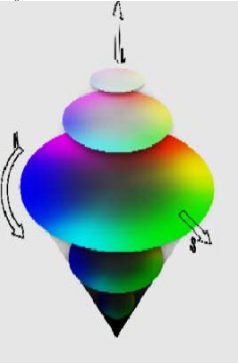
\includegraphics[scale=0.3]{espaco_hsi.png}
			\caption{Espaço de cores do modelo de cores HSI. fonte:\cite{ibraheem2012understanding} }
		\end{figure}
	\end{center}
	
	
\bibliographystyle{IEEEtranS}
\bibliography{bibliography}
\end{document}

